
\section{Introduction}

Many geometric algorithms implemented in \cgal\ are incremental, and thus their
speed is dependent on the order of insertion.  This package provides sorting
algorithms that may considerably improve running times of such
algorithms.

The rationale is to sort objects along a space-filling curve 
so that two
objects close geometrically will be close in the insertion order with high
probability.  That way, parts of a data structure that will be looked at during
an insertion will probably have been looked at in a recent insertion, and thus
probably will be in cache memory instead of main memory.
As another side-effect, these sorting functions usually improve memory locality
of the data structures produced by incremental algorithms, sometimes leading to
speed ups in other algorithm using these data structures.

Some algorithms have a good complexity under randomized hypotheses which
contradicts the idea of sorting the input using any sorting criterion.
In such a case, it is possible to introduce just a bit of randomness 
to be able to combine the good randomized complexity and the
good effects of locality \cite{acr-icb-03}.


The predicates used by this package are comparisons between coordinates,
thus there is no robustness issue involved here, for example to choose the
arithmetic of the kernel.


\section{Hilbert Sorting\label{sec:hilbert_sorting}}


In 2D, one can construct a space filling curve, that is a mapping $f$ of $[0,1]$
to the unit square $[0,1]^2$, such that $f(0)=(0,0)$ and $f(1)=(1,0)$ 
 in the following way:
the unit square is subdivided in four such that\\
\begin{quote}
$f([0,\frac{1}{4}])=[0,\frac{1}{2}]^2$, 
$f([\frac{1}{4},\frac{1}{2}])=[0,\frac{1}{2}]\times[\frac{1}{2},1]$,
$f([\frac{1}{2},\frac{3}{4}])=[\frac{1}{2},1]^2$,
and 
$f([\frac{3}{4},1])=[\frac{1}{2},1]\times[0,\frac{1}{2}].$\\
$f(\frac{1}{4})=(0,\frac{1}{2})$\\
$f(\frac{1}{2})=(\frac{1}{2},\frac{1}{2})$, and
$f(\frac{3}{4})=(1,\frac{1}{2})$.
\end{quote}

Then each square is subdivided in the same way recursively.
Figure~\ref{Spatial_sorting_fig_Hilbert8} illustrates this process.

\begin{figure}
\begin{ccHtmlOnly}
<center>
<img border=0 src="./fig/Hilbert8.gif" align=middle>
</center>
\end{ccHtmlOnly} 
\begin{ccTexOnly}
\begin{center}
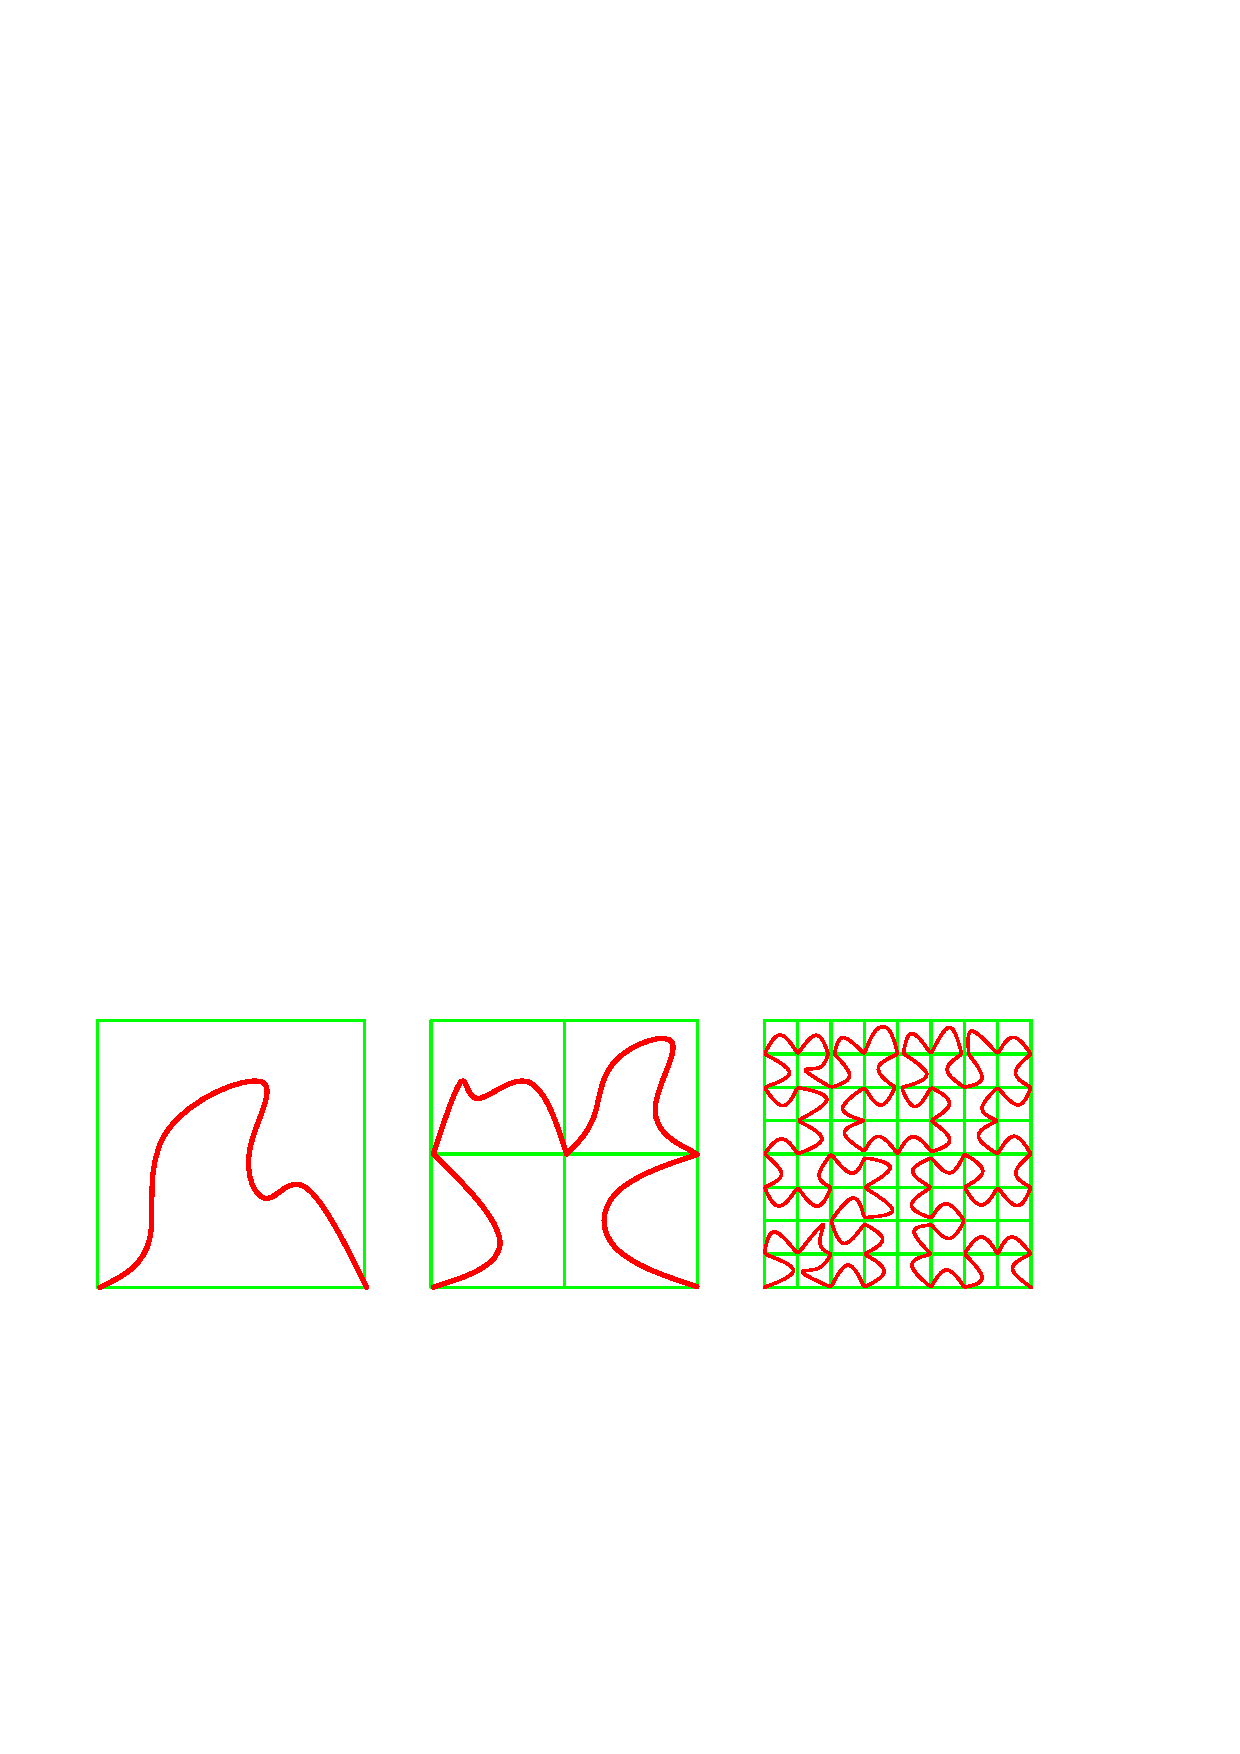
\includegraphics[width=11.5cm]{Spatial_sorting/fig/Hilbert8}
\end{center}
\end{ccTexOnly}
\caption{Hilbert mapping
\label{Spatial_sorting_fig_Hilbert8}}
\end{figure}

Now given a set of 2D points, they can be sorted in the order they have on such
a space filling curve as illustrated in Figure~\ref{Spatial_sorting_fig_Hilbert_middle} :

\begin{figure}[h]
\begin{ccHtmlOnly}
<center>
<img border=0 src="./fig/Hilbert-middle.gif" align=middle>
</center>
\end{ccHtmlOnly} 
\begin{ccTexOnly}
\begin{center}
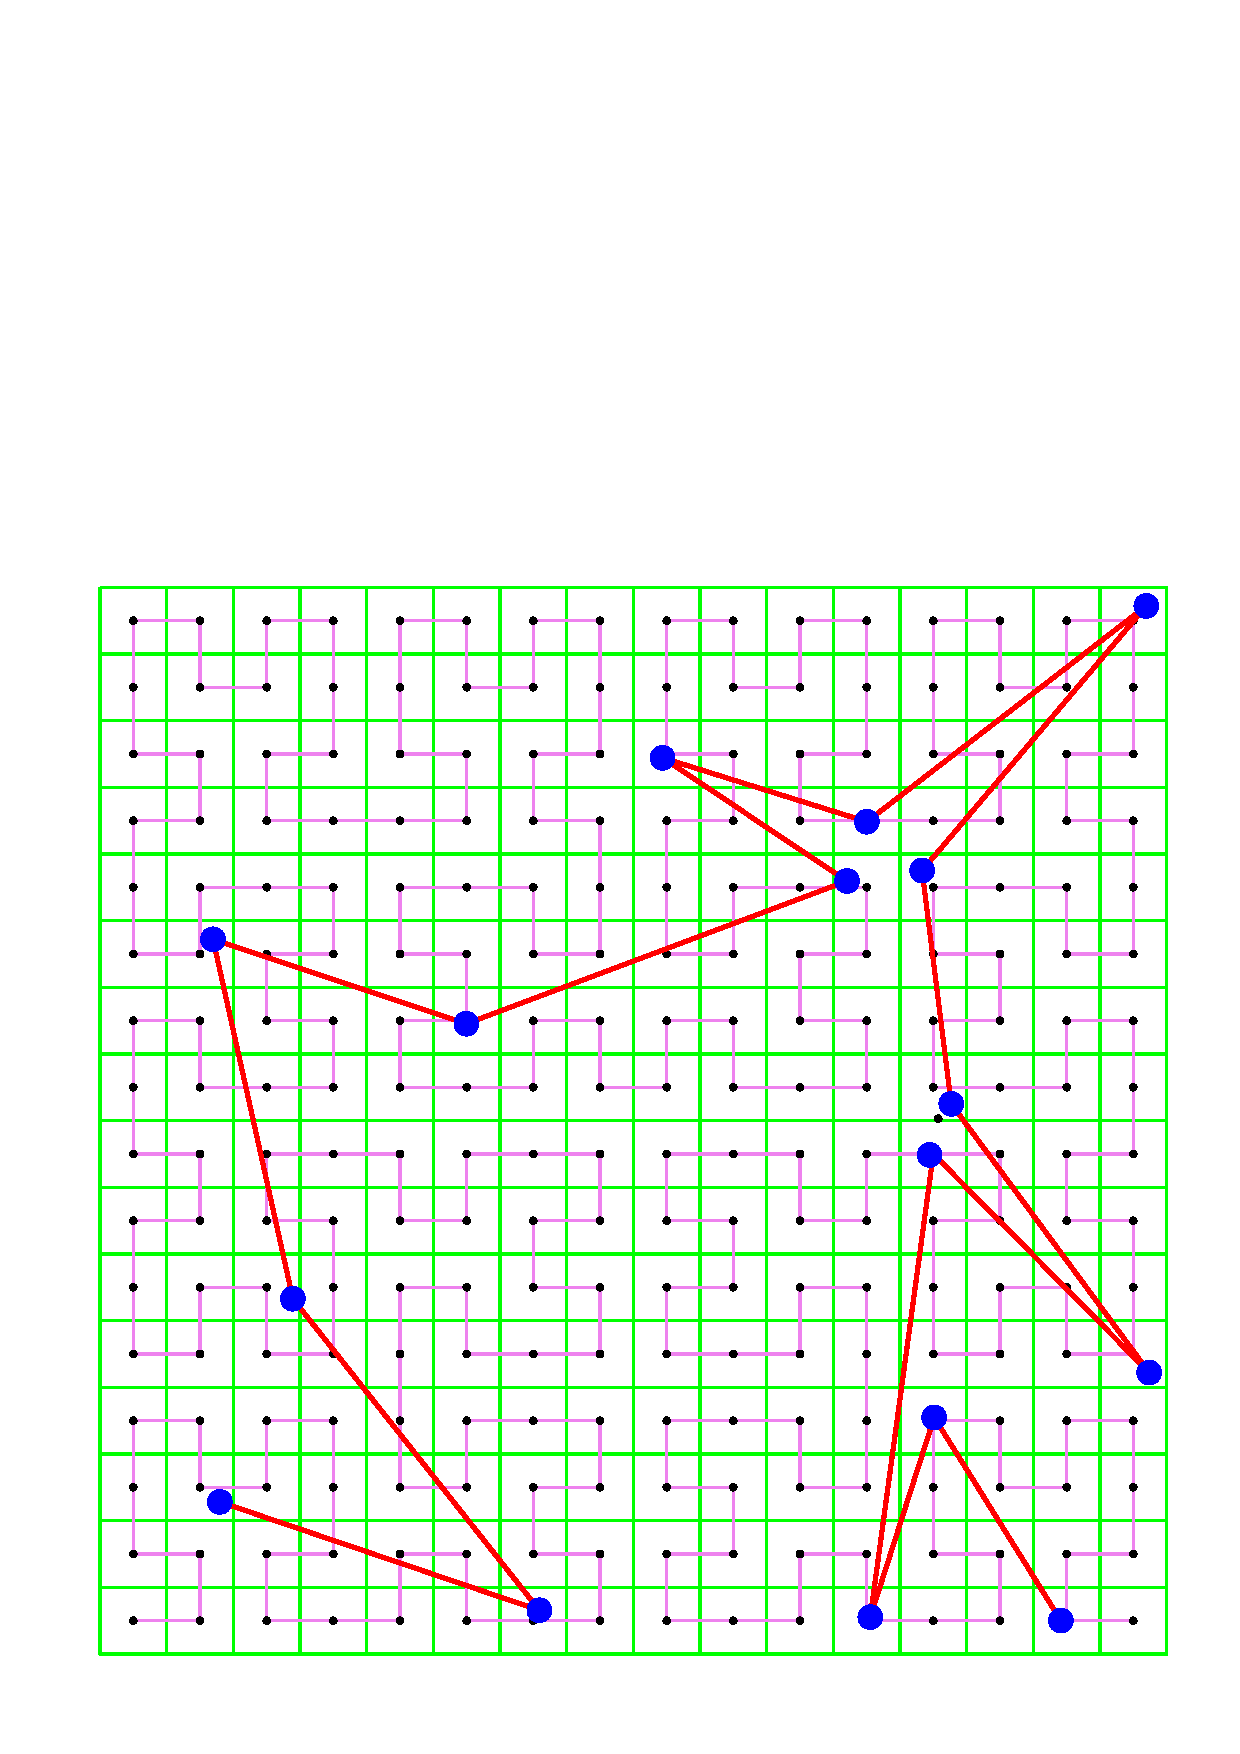
\includegraphics[width=6.5cm]{Spatial_sorting/fig/Hilbert-middle}
\end{center}
\end{ccTexOnly}
\caption{Hilbert sort with middle policy
\label{Spatial_sorting_fig_Hilbert_middle}}
\end{figure}

\begin{ccTexOnly}
\newpage
\end{ccTexOnly}

\subsection{Examples}

The code to use Hilbert sort is as simple as the following example:

\ccIncludeExampleCode{Spatial_sorting/hilbert.cpp}


If instead of subdividing the square in a fixed way at its middle point,
 as above, we subdivide it
by splitting at the median point (in $x$ or $y$ directions alternating),
we construct a 2-d tree adapted to the point set. This tree can be visited in a
similar manner and we get also a suitable ordering of the points
(see Figure~\ref{Spatial_sorting_fig_Hilbert_median}).


\begin{figure}[t]
\begin{ccHtmlOnly}
<center>
<img border=0 src="./fig/Hilbert-median.gif" align=middle>
</center>
\end{ccHtmlOnly} 
\begin{ccTexOnly}
\begin{center}
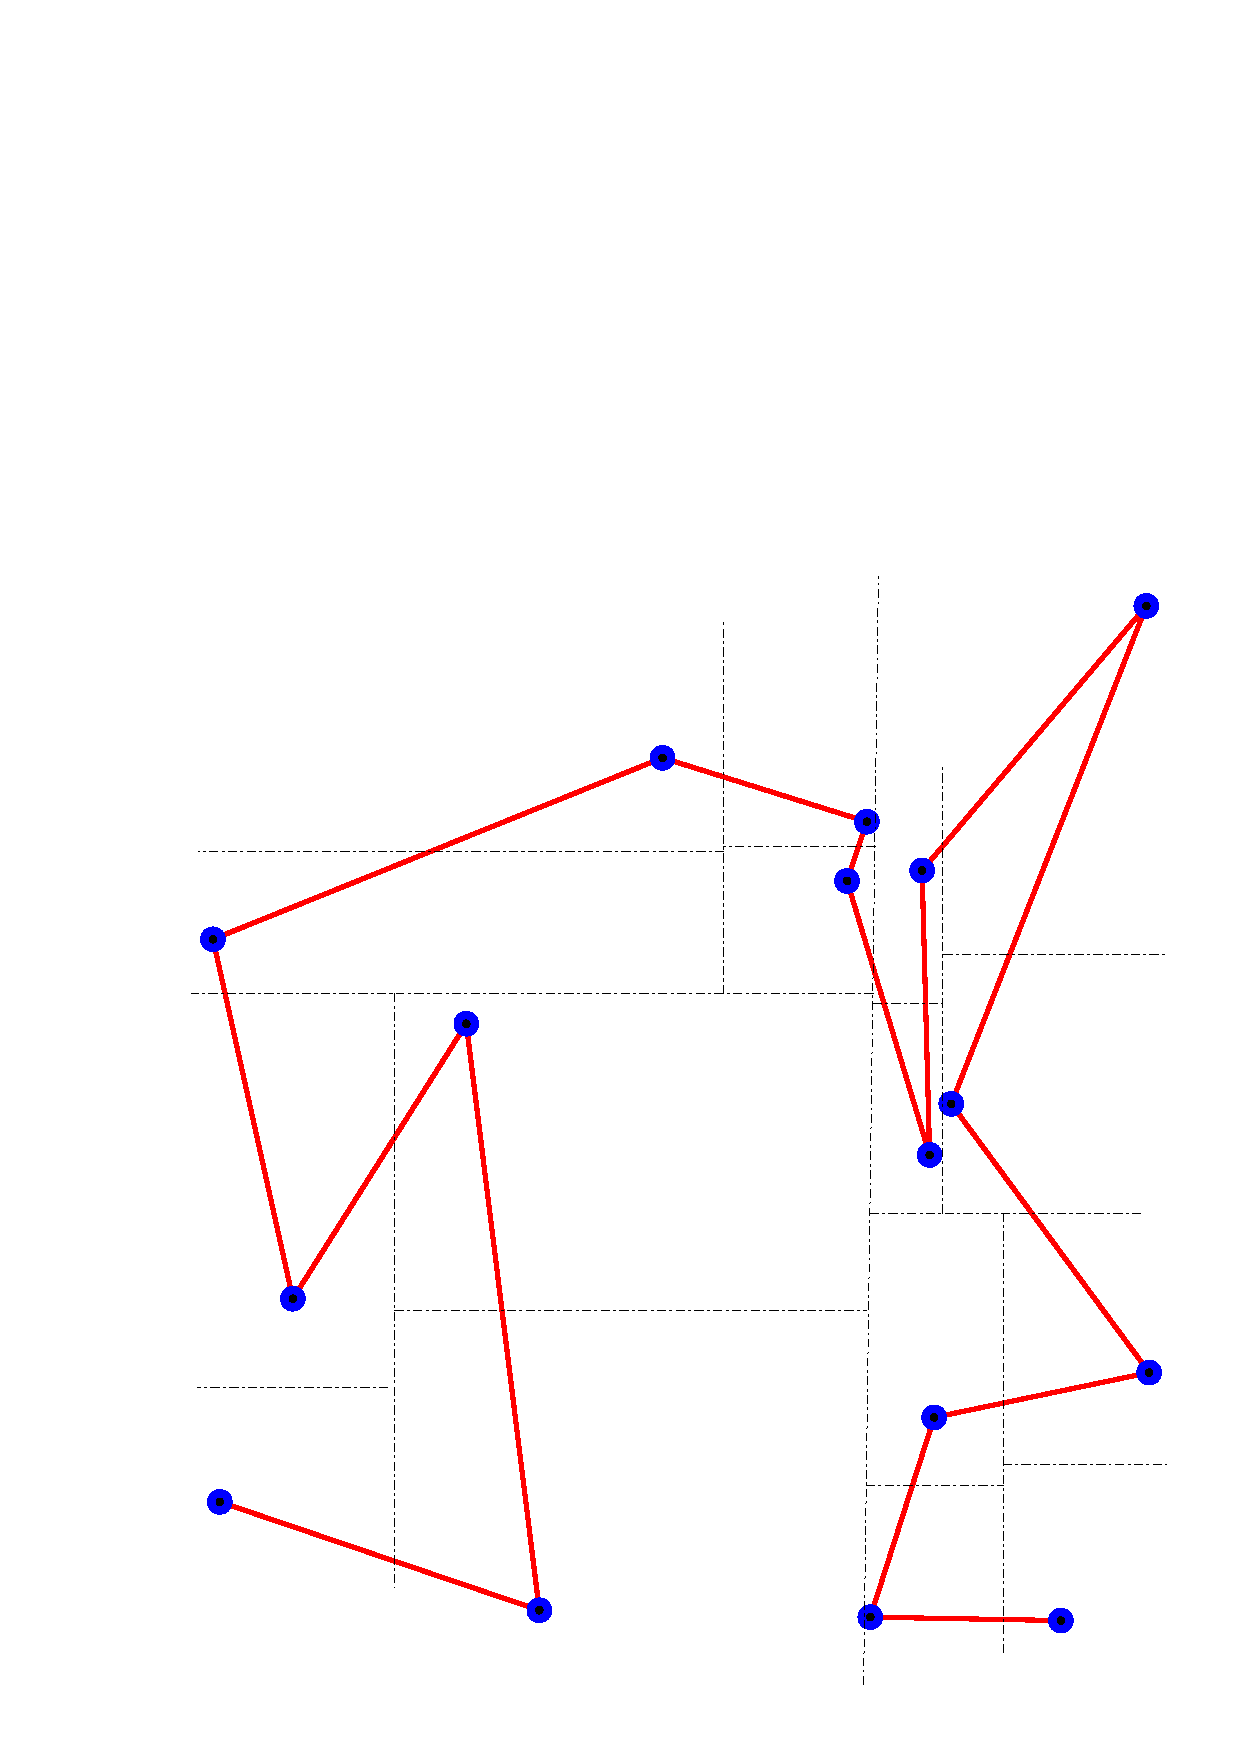
\includegraphics[width=6.5cm]{Spatial_sorting/fig/Hilbert-median}
\end{center}
\end{ccTexOnly}
\caption{Hilbert sort with median policy
\label{Spatial_sorting_fig_Hilbert_median}}
\end{figure}


\cgal\ provides Hilbert sorting for points in 2D, 3D and higher dimensions,
in the middle and the median policies.

The middle policy is easier to analyze, and is interesting in practice
for well distributed set of points in small dimension (if the number
of points is really smaller than $2^d$).
The median policy should be prefered for high dimension or if 
the point set distribution is not regular (or unknown).
Since the median policy cannot be much worse than the middle
policy, while the converse can happen, the median policy is the
default behavior.
Most theoretical results are using the middle policy
\cite{acr-icb-03,b-aahsf-71,bg-sfche-89,pb-scpts-89}.


This other example illustrates the use of the two different policies


\ccIncludeExampleCode{Spatial_sorting/hilbert_policies.cpp}


\section{Spatial Sorting\label{sec:spatial_sorting}}

Hilbert sort cannot be used directly before feeding a randomized algorithm.
Thus, the trick is to organize the point set in random buckets of increasing
sizes, Hilbert sort being used only inside a bucket.

It has been proved, in the context of Delaunay triangulation, that
such an order provides enough randomness to combine the advantages of a random
 order and a space filling curve order \cite{acr-icb-03}.


\cgal\ provides spatial sorting for points in 2D, 3D and higher dimensions,
with the middle and the median policies for Hilbert sort in the buckets.

\subsection{Basic Example}

The following example shows that, on particular input, spatial sort
runs much faster than a bad order or than Hilbert sort (below results
with release mode compilation on a 1.8GHz processor).
\begin{verbatim}
$ ./small_example_delaunay_2 
10000 points on a parabola
  Delaunay without spatial sort...         done in 6.33443 seconds.
  Delaunay with median hilbert sort...     done in 0.822975 seconds.
  Delaunay with median spatial sort...     done in 0.022415 seconds.
\end{verbatim}

\ccIncludeExampleCode{Spatial_sorting/small_example_delaunay_2.cpp}

%Next example describes how a traits class different than CGAL Kernel can be
%used to sort a container of handle on points instead of points directly.
%\ccIncludeExampleCode{Spatial_sorting/sort_indices.cpp}

\subsection{Using Your Own Point Type}
If you want to sort points of your own point type,
you only have to provide functors that compare
the \ccc{x} and \ccc{y} coordinates of your points. Note that in case you simply want
to associate an extra information to your point you might consider the example of Section
\ref{sec:sort_any_type_2}
as an alternative.

\ccIncludeExampleCode{Spatial_sorting/myPoint.cpp}

\subsection{Sorting Arbitrary Types}
\label{sec:sort_any_type}
The spatial sorting traits class provides a point type and
functors for comparing, for example, the \ccc{x}-coordinates
of two points.
%
If you want to sort something else than just points, for example
a sequence of tuples containing a point,  or a sequence of indices
in a vector of points, you need another level of indirection.
%
We provide the spatial sorting traits class adapters which are templated by
another spatial sorting traits class, and a 
\ccAnchor{http://www.boost.org/doc/libs/release/libs/property_map/index.html}{property map}.
which allows to obtain a point from whatever you want to sort. 

The following examples illustrate the usage of these traits class adapters.

\subsubsection{Sorting Using Pairs of Points and Integers}
\label{sec:sort_any_type_2}
In this example program, the sorted sequence of points is retrieved 
using a vector of pairs of points and integers.
\ccIncludeExampleCode{Spatial_sorting/sp_sort_using_property_map_2.cpp}

\subsubsection{Sorting Using Indices of Points}
In this example program, the sorted sequence of points is retrieved 
using the indices of the points in a vector of points.
\ccIncludeExampleCode{Spatial_sorting/sp_sort_using_property_map_3.cpp}

\subsubsection{Sorting Using Indices of Pairs of Points and Integers}
In this example program, the sorted sequence of points is retrieved 
using the indices of the points in a vector of pairs of points and integers.
\ccIncludeExampleCode{Spatial_sorting/sp_sort_using_property_map_d.cpp}



